\documentclass[12pt,a4paper]{report}
\usepackage[utf8]{inputenc}
\usepackage[T1]{fontenc}
\usepackage[bahasa]{babel}
\usepackage{graphicx}
\usepackage{float}
\usepackage{tikz}
\usetikzlibrary{shapes,arrows,positioning,fit,calc}
\usepackage{booktabs}
\usepackage{longtable}
\usepackage{listings}
\usepackage{hyperref}
\usepackage{xcolor}
\usepackage{setspace}
\usepackage{array}
\usepackage{amssymb}
\usepackage{microtype}
\usepackage{seqsplit}
\usepackage[compact]{titlesec}
\titleformat{\chapter}[display]{\normalfont\huge\bfseries}{\chaptertitlename\ \thechapter}{12pt}{\Huge}
\titlespacing*{\chapter}{0pt}{-20pt}{20pt}
% \geometry{margin=2cm, bottom=2cm}
\usepackage[a4paper,left=2cm,right=2cm]{geometry}
\savegeometry{titlepage}
\geometry{top=3cm,bottom=3cm,left=2.5cm,right=2.5cm}
% Pengaturan kutipan artikel
\onehalfspacing

\hypersetup{
    colorlinks=true,
    linkcolor=black,
    citecolor=black,
    urlcolor=blue,
    pdftitle={Laporan Progres Proyek Akhir TiketKita},
    pdfauthor={Kelompok 11}
}

\begin{document}

%======================================================================
% HALAMAN JUDUL / COVER
%======================================================================
\begin{titlepage}
    \centering
    \vspace*{0cm}

    {\large\bfseries Laporan Progres Proyek Akhir\\[0.2cm]
    Platform Tiket Online TiketKita\par}
    
    \vspace{0.65cm}
    
\includegraphics[width=8cm]{logodepart.png}

    \vspace{0.65cm}
    {\normalsize\bfseries Mata Kuliah\par}
    {\normalsize Sistem Basis Data\par}

    \vspace{0.45cm}
    {\normalsize\bfseries Dosen Pengampu\par}
    {\normalsize Dr. Arief Kurniawan, S.T., M.T.\par}

    \vspace{0.75cm}
    {\normalsize\bfseries Disusun oleh:\par}
    {\normalsize Kelompok 11\par}

    \vspace{0.45cm}
    \small
    \begin{tabular}{|l|l|}
        \hline
        \textbf{Nama} & \textbf{NRP} \\
        \hline
        Aisyah Nuurii Winsetyowati & 5024241008 \\
        Atika Najwa Azzahra & 5024241091 \\
        Yuke Brilliant Hestiavin & 5024241016 \\
        \hline
    \end{tabular}
    \normalsize

    \vspace{0.9cm}
    {\normalsize\bfseries Departemen Teknik Komputer\par}
    {\normalsize Institut Teknologi Sepuluh Nopember\par}
    {\normalsize Surabaya, 18 Mei 2026\par}
\end{titlepage}

%======================================================================
% KATA PENGANTAR
%======================================================================
\chapter*{Kata Pengantar}
\addcontentsline{toc}{chapter}{Kata Pengantar}

Puji syukur kami panjatkan ke hadirat Tuhan Yang Maha Esa atas segala rahmat dan karunia-Nya, sehingga laporan progres proyek akhir mata kuliah Sistem Basis Data ini dapat kami selesaikan tepat waktu. Laporan ini disusun sebagai bagian dari tugas akhir yang menuntut implementasi nyata dari konsep basis data relasional, mulai dari perancangan skema, normalisasi, hingga penerapan transaksi pada sistem aplikasi yang utuh.

Laporan ini memuat progres pengembangan TiketKita, sebuah platform tiket online yang dibangun untuk mengelola event, tipe tiket, pemesanan, hingga pembayaran. Pada tahap progres ini kami telah menyelesaikan REST API backend dengan arsitektur berlapis serta dashboard admin untuk pengelolaan data. Dokumen ini menjelaskan latar belakang, landasan teori, perancangan basis data, implementasi sistem, serta hasil pengujian sejauh ini.

Kami menyampaikan terima kasih yang sebesar-besarnya kepada Bapak Dr. Arief Kurniawan, S.T., M.T. selaku dosen pengampu mata kuliah Sistem Basis Data atas bimbingan, arahan, dan masukan yang sangat berharga selama proses pengerjaan proyek ini. Tidak lupa kami berterima kasih kepada rekan-rekan dan semua pihak yang telah memberikan dukungan sehingga laporan ini dapat tersusun. Kritik dan saran yang membangun sangat kami harapkan demi penyempurnaan laporan dan proyek ini ke depan.

\vspace{1cm}
\begin{flushright}
Surabaya, 18 Mei 2026\\[1cm]
Tim Kelompok 11
\end{flushright}

%======================================================================
% DAFTAR ISI / GAMBAR / TABEL
%======================================================================
\tableofcontents
\listoffigures
\listoftables

%======================================================================
% BAB I PENDAHULUAN
%======================================================================
\chapter{Pendahuluan}

\section{Latar Belakang}
Industri hiburan dan pertunjukan di Indonesia tumbuh pesat dalam beberapa tahun terakhir, mulai dari konser musik, festival, seminar, hingga ajang olahraga. Pertumbuhan tersebut mendorong meningkatnya kebutuhan masyarakat akan platform tiket online yang dapat diakses dengan mudah, aman, dan transparan. Penjualan tiket secara digital memberikan banyak keuntungan, antara lain efisiensi proses pemesanan, kemudahan pembayaran daring, serta pengelolaan data peserta yang lebih rapi bagi penyelenggara acara.

Proyek TiketKita dikembangkan sebagai tugas akhir mata kuliah Sistem Basis Data dengan fokus pada penerapan konsep basis data relasional menggunakan MySQL secara langsung tanpa bantuan ORM. Pendekatan tanpa ORM dipilih agar setiap perintah SQL ditulis secara eksplisit, sehingga konsep seperti kunci utama, kunci asing, normalisasi, indeks, dan transaksi benar-benar dipahami dan diimplementasikan dengan sadar. Melalui proyek ini kami berlatih merancang skema basis data dari kebutuhan bisnis, kemudian mengintegrasikannya dengan REST API berbasis Node.js dan TypeScript serta dashboard administrator berbasis Next.js.

\section{Rumusan Masalah}
Berdasarkan latar belakang di atas, rumusan masalah yang diangkat dalam laporan progres ini adalah sebagai berikut.
\begin{enumerate}
    \item Bagaimana merancang skema basis data relasional yang efisien untuk platform tiket online?
    \item Bagaimana mengimplementasikan transaksi database untuk menghindari race condition pada pemesanan tiket?
    \item Bagaimana membangun REST API yang terstruktur dengan arsitektur Controller-Service-Repository?
    \item Bagaimana menyediakan antarmuka admin yang informatif untuk pengelolaan event dan monitoring transaksi?
\end{enumerate}

\section{Tujuan}
Tujuan dari pengerjaan proyek TiketKita pada tahap progres ini adalah sebagai berikut.
\begin{enumerate}
    \item Merancang dan mengimplementasikan skema basis data relasional dengan 11 tabel yang ternormalisasi.
    \item Mengimplementasikan mekanisme transaksi MySQL untuk menjamin konsistensi data pemesanan tiket.
    \item Membangun REST API backend dengan Node.js, TypeScript, dan Express menggunakan raw SQL.
    \item Membangun dashboard admin dengan Next.js untuk pengelolaan event, tiket, order, dan pembayaran.
\end{enumerate}

\section{Manfaat}
Pengerjaan proyek ini diharapkan memberikan manfaat sebagai berikut.
\begin{enumerate}
    \item Manfaat akademis: memberi pemahaman mendalam mengenai implementasi nyata konsep basis data relasional, normalisasi, dan transaksi pada studi kasus aplikasi yang utuh.
    \item Manfaat teknis: memberi pengalaman membangun sistem full-stack dengan arsitektur berlapis yang terstruktur, mulai dari migrasi basis data, REST API, hingga antarmuka admin.
    \item Manfaat praktis: menghasilkan prototipe platform tiket online yang dapat dikembangkan lebih lanjut menjadi produk siap pakai bagi penyelenggara event.
\end{enumerate}

\section{Ruang Lingkup}
Pada tahap progres ini, fitur-fitur yang sudah diimplementasikan meliputi REST API backend dengan 11 modul fungsional yang didukung oleh 11 tabel basis data, dashboard admin dengan 10 halaman pengelolaan, sistem migrasi basis data beserta seed data, serta dokumentasi API otomatis menggunakan Scalar. Seluruh komponen ini sudah dapat menjalankan alur dasar pemesanan, mulai dari otentikasi pengguna, pembuatan event dan tiket, pemesanan oleh pengguna, hingga konfirmasi pembayaran secara simulatif.

Sebaliknya, beberapa bagian belum dikerjakan pada tahap ini dan menjadi rencana pengembangan selanjutnya. Bagian tersebut meliputi frontend publik atau customer-facing, integrasi payment gateway nyata, deployment ke environment production, serta fitur CRUD promo codes pada dashboard admin yang masih dalam pengerjaan. Lingkup laporan ini dibatasi pada hasil yang sudah dapat diverifikasi pada tahap progres dan landasan teori yang mendasarinya.

%======================================================================
% BAB II LANDASAN TEORI
%======================================================================
\chapter{Landasan Teori}

\section{Basis Data Relasional}
Basis data relasional adalah model basis data yang merepresentasikan data dalam bentuk tabel dua dimensi dengan baris dan kolom, dimana setiap baris merupakan tuple atau record dan setiap kolom merupakan atribut. Konsep ini diperkenalkan oleh E.F. Codd dan menjadi dasar dari sebagian besar sistem manajemen basis data modern atau Relational Database Management System (RDBMS). Pada model relasional, hubungan antar entitas direpresentasikan melalui kunci, yaitu kunci utama (primary key) untuk identifikasi unik dan kunci asing (foreign key) untuk merujuk ke tabel lain. MySQL dipilih sebagai RDBMS pada proyek TiketKita karena bersifat open source, banyak digunakan di industri, mendukung transaksi ACID melalui mesin penyimpanan InnoDB, serta memiliki dokumentasi dan dukungan komunitas yang luas.

\section{Entity-Relationship Diagram}
Entity-Relationship Diagram (ERD) adalah diagram konseptual yang digunakan untuk menggambarkan struktur basis data sebelum diterjemahkan ke dalam skema relasional. ERD memodelkan dunia nyata dalam bentuk entitas, atribut, dan relasi. Entitas merepresentasikan objek atau konsep, misalnya pengguna, event, atau tiket. Atribut adalah karakteristik yang melekat pada entitas, sedangkan relasi adalah hubungan antar entitas. Relasi memiliki kardinalitas yang menggambarkan jumlah keterhubungan, yaitu satu ke satu (1:1), satu ke banyak (1:N), dan banyak ke banyak (M:N). Kardinalitas ini menentukan bagaimana tabel dirancang, termasuk kebutuhan akan tabel jembatan untuk relasi banyak ke banyak.

\section{Normalisasi Basis Data}
Normalisasi adalah proses sistematis untuk mengorganisasi data pada basis data relasional agar terbebas dari anomali penyisipan, pembaruan, dan penghapusan, serta meminimalkan redudansi. Bentuk normal pertama (1NF) mensyaratkan setiap kolom bernilai atomik dan tidak ada grup berulang. Bentuk normal kedua (2NF) menambahkan syarat ketergantungan fungsional penuh terhadap seluruh kunci utama, sehingga atribut non-kunci harus bergantung pada keseluruhan kunci komposit. Bentuk normal ketiga (3NF) lebih ketat lagi dengan menghilangkan ketergantungan transitif, yaitu atribut non-kunci yang bergantung pada atribut non-kunci lain. Pada perancangan basis data TiketKita, prinsip normalisasi diterapkan untuk memisahkan entitas seperti pengguna, event, venue, kategori, tiket, order, dan pembayaran ke dalam tabel terpisah dengan kunci asing yang sesuai.

\section{REST API}
Representational State Transfer (REST) adalah gaya arsitektur untuk membangun layanan web yang memanfaatkan protokol HTTP secara semantik. REST API bersifat stateless, artinya setiap permintaan dari klien harus berisi seluruh informasi yang diperlukan untuk diproses tanpa bergantung pada state sesi di sisi server. Operasi pada sumber daya dipetakan ke metode HTTP standar, yaitu GET untuk mengambil data, POST untuk membuat data baru, PUT atau PATCH untuk memperbarui data, dan DELETE untuk menghapus data. Pertukaran data umumnya menggunakan format JSON karena ringan dan mudah diproses oleh berbagai bahasa pemrograman. Pada TiketKita, REST API digunakan sebagai antarmuka utama antara frontend dashboard dan basis data MySQL, dengan struktur endpoint yang dikelompokkan per modul fungsional.

\section{Transaksi dan Race Condition}
Transaksi pada basis data adalah serangkaian operasi yang dieksekusi sebagai satu kesatuan logis dan harus memenuhi prinsip ACID, yaitu Atomicity, Consistency, Isolation, dan Durability. Pada platform tiket online, race condition dapat terjadi ketika dua atau lebih proses pemesanan mengakses dan memperbarui stok tiket yang sama secara bersamaan, sehingga jumlah tiket yang terjual berpotensi melebihi kuota yang tersedia. Skenario ini sangat berbahaya karena dapat menimbulkan oversold dan kerugian operasional. Solusi yang umum digunakan adalah penguncian baris dengan perintah \texttt{SELECT ... FOR UPDATE} untuk memastikan baris stok dikunci selama transaksi, atau pembaruan atomik dengan kondisi pada klausa \texttt{WHERE}, misalnya \texttt{UPDATE ticket\_types SET available = available - qty WHERE id = ? AND available >= qty}. Pendekatan kedua memanfaatkan jumlah baris terdampak (\texttt{affectedRows}) sebagai indikator keberhasilan, sehingga jika stok tidak mencukupi maka transaksi langsung di-rollback.

%======================================================================
% BAB III ANALISIS DAN PERANCANGAN
%======================================================================
\chapter{Analisis dan Perancangan}

\section{Deskripsi Sistem}
TiketKita adalah platform tiket online yang memungkinkan pengguna menelusuri event, memesan tiket, dan melakukan pembayaran secara simulatif dalam satu sistem terintegrasi. Sistem dibangun dengan arsitektur berlapis yang memisahkan tanggung jawab antara basis data, layanan API, dan antarmuka pengguna, sehingga memudahkan pengembangan dan pengujian setiap komponen secara terpisah. Pada tahap progres ini, fokus pengembangan diarahkan pada penyelesaian REST API backend dan dashboard administrator yang menjadi tulang punggung pengelolaan data event dan transaksi.

Alur penggunaan secara garis besar dimulai dari registrasi pengguna, kemudian pengguna dapat menjelajahi daftar event yang sudah dipublikasikan, memilih tipe tiket yang diinginkan, dan melanjutkan ke proses checkout dengan opsi penggunaan kode promo. Setelah order dibuat, pengguna mengkonfirmasi pembayaran melalui metode yang dipilih, lalu sistem akan menandai tiket sebagai terkonfirmasi. Di sisi administrator, dashboard menyediakan akses untuk mengelola event, tipe tiket, order, pembayaran, kategori, venue, serta melihat statistik ringkasan platform.

\section{Fitur Utama}
\begin{itemize}
    \item Registrasi dan autentikasi pengguna dengan JWT.
    \item Verifikasi email dan reset password.
    \item Penelusuran dan detail event (filter kategori, pencarian judul).
    \item Pemesanan tiket dengan validasi stok real-time.
    \item Checkout dengan kode promo (persentase atau nominal).
    \item Simulasi pembayaran multi-metode (e-wallet, VA, QRIS, kartu kredit, transfer bank).
    \item Wishlist event favorit.
    \item Auto-cancel order yang kedaluwarsa (setiap 60 detik).
    \item Dashboard admin: statistik, manajemen event/tiket/order/pembayaran/kategori/venue.
    \item Dokumentasi API interaktif via Scalar di \texttt{/api/docs}.
\end{itemize}

\section{Arsitektur Sistem}
Arsitektur TiketKita mengadopsi pola tiga lapis (3-tier) yang memisahkan tanggung jawab penyimpanan data, logika aplikasi, dan antarmuka pengguna. Lapisan database menggunakan MySQL 8.0 sebagai sumber data tunggal yang menyimpan seluruh entitas sistem. Lapisan backend dibangun dengan Node.js dan Express yang berkomunikasi ke database menggunakan driver mysql2. Lapisan frontend menggunakan Next.js sebagai dashboard administrator yang berinteraksi dengan backend melalui REST API berformat JSON.

\begin{figure}[h]
\centering
\begin{tikzpicture}[node distance=2.5cm, auto]
  \tikzstyle{block} = [rectangle, draw, fill=blue!10, text width=3.5cm, text centered, minimum height=1.2cm, rounded corners]
  \tikzstyle{arrow} = [thick,->,>=stealth]
  \node [block] (db) {MySQL 8.0\\(Database Layer)};
  \node [block, right of=db, node distance=5.5cm] (api) {Node.js + Express\\(Backend Layer)};
  \node [block, right of=api, node distance=6.5cm] (fe) {Next.js 16\\(Frontend Layer)};
  \draw [arrow] (db) -- node[above]{\small mysql2} (api);
  \draw [arrow] (api) -- node[above]{\small REST API} (fe);
  \draw [arrow,<->] (api) -- (db);
  \draw [arrow,<->] (fe) -- (api);
\end{tikzpicture}
\caption{Arsitektur 3-Tier Sistem TiketKita}
\label{fig:arsitektur}
\end{figure}

\section{Entity-Relationship Diagram}
Basis data TiketKita terdiri dari sebelas tabel utama yang saling berelasi. Gambar \ref{fig:erd-lengkap} menampilkan ERD lengkap yang merangkum seluruh entitas, atribut kunci, dan relasi antar entitas dalam satu diagram. Diagram ini dibuat menggunakan Mermaid kemudian diekspor ke format gambar untuk disisipkan ke dalam laporan.

\begin{figure}[H]
\centering
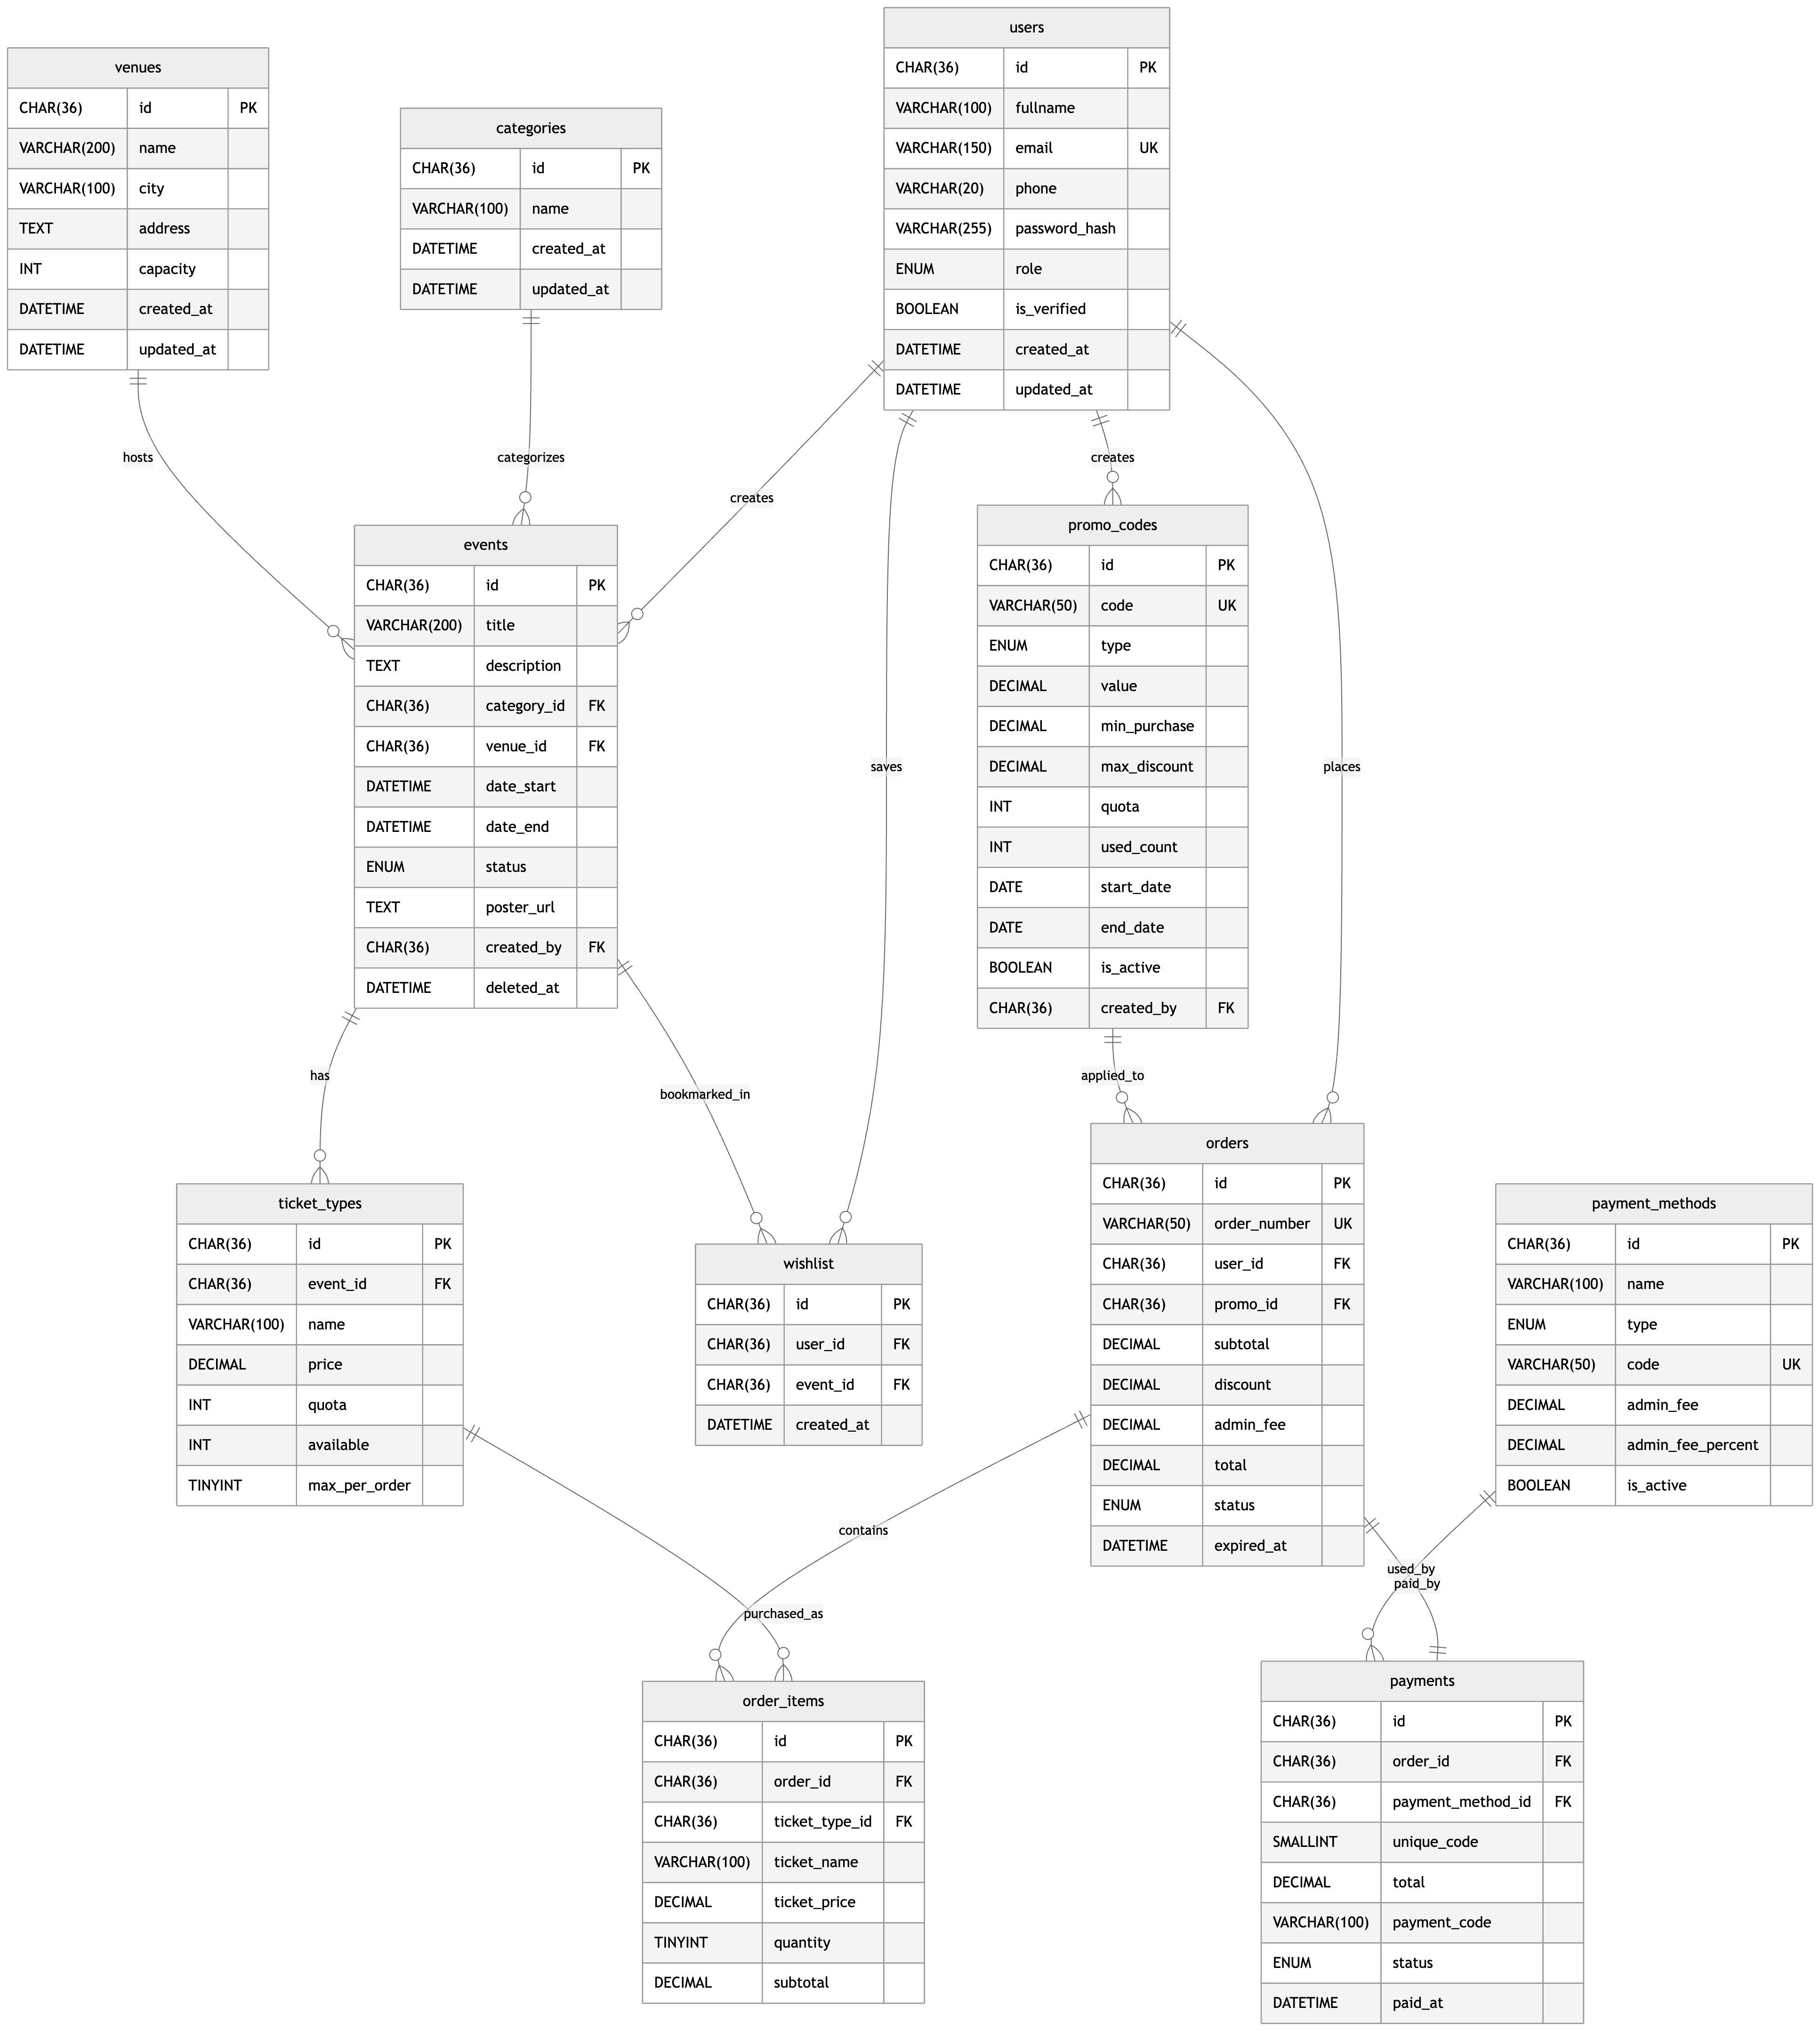
\includegraphics[width=\textwidth,keepaspectratio]{erd.png}
\caption{ERD Lengkap Basis Data TiketKita}
\label{fig:erd-lengkap}
\end{figure}

\noindent Sumber Mermaid yang dipakai untuk merender diagram di atas tercantum pada Listing \ref{lst:erd-mermaid}.

\section{Skema Relasi dan Detail Setiap Entitas}
Bagian ini menjabarkan struktur lengkap setiap entitas pada basis data TiketKita. Setiap tabel ditampilkan dalam bentuk daftar kolom beserta tipe data dan keterangan, sehingga memudahkan pembaca memahami detail skema tanpa perlu membaca berkas migrasi. Seluruh entitas menggunakan tipe \texttt{CHAR(36)} sebagai kunci utama berbasis UUID dan menyimpan stempel waktu standar \texttt{created\_at} dan \texttt{updated\_at} kecuali pada tabel yang hanya bersifat pencatatan tunggal.

\subsection{Tabel users}
Tabel \texttt{users} menyimpan data akun pengguna dan administrator beserta status verifikasi dan kode reset password.

\begin{longtable}{p{3.6cm} p{3.6cm} p{8.5cm}}
\caption{Struktur Tabel users} \label{tab:users} \\
\toprule
\textbf{Kolom} & \textbf{Tipe} & \textbf{Keterangan} \\
\midrule
\endfirsthead
\toprule
\textbf{Kolom} & \textbf{Tipe} & \textbf{Keterangan} \\
\midrule
\endhead
\bottomrule
\endfoot
id            & CHAR(36)     & Kunci utama berbasis UUID. \\
fullname      & VARCHAR(100) & Nama lengkap pengguna. \\
email         & VARCHAR(150) & Email unik untuk login. \\
phone         & VARCHAR(20)  & Nomor telepon, opsional. \\
password\_hash & VARCHAR(255) & Hash password (bcrypt). \\
role          & ENUM         & Nilai \texttt{user} atau \texttt{admin}. \\
is\_verified  & BOOLEAN      & Status verifikasi email. \\
verification\_code              & VARCHAR(10) & Kode verifikasi email. \\
\seqsplit{verification\_code\_expires\_at} & DATETIME    & Kedaluwarsa kode verifikasi. \\
reset\_code                     & VARCHAR(10) & Kode reset password. \\
\seqsplit{reset\_code\_expires\_at}     & DATETIME     & Kedaluwarsa kode reset. \\
created\_at   & DATETIME     & Waktu pembuatan record. \\
updated\_at   & DATETIME     & Waktu pembaruan terakhir. \\
\end{longtable}

\subsection{Tabel venues}
Tabel \texttt{venues} menyimpan informasi lokasi penyelenggaraan event beserta kapasitas total.

\begin{longtable}{p{3.6cm} p{3.6cm} p{8.5cm}}
\caption{Struktur Tabel venues} \label{tab:venues} \\
\toprule
\textbf{Kolom} & \textbf{Tipe} & \textbf{Keterangan} \\
\midrule
\endfirsthead
\toprule
\textbf{Kolom} & \textbf{Tipe} & \textbf{Keterangan} \\
\midrule
\endhead
\bottomrule
\endfoot
id          & CHAR(36)      & Kunci utama berbasis UUID. \\
name        & VARCHAR(200)  & Nama venue. \\
city        & VARCHAR(100)  & Kota tempat venue berada. \\
address     & TEXT          & Alamat lengkap. \\
capacity    & INT UNSIGNED  & Kapasitas total venue. \\
created\_at & DATETIME      & Waktu pembuatan record. \\
updated\_at & DATETIME      & Waktu pembaruan terakhir. \\
\end{longtable}

\subsection{Tabel categories}
Tabel \texttt{categories} menyimpan kategori event seperti konser, festival, atau seminar.

\begin{longtable}{p{3.6cm} p{3.6cm} p{8.5cm}}
\caption{Struktur Tabel categories} \label{tab:categories} \\
\toprule
\textbf{Kolom} & \textbf{Tipe} & \textbf{Keterangan} \\
\midrule
\endfirsthead
\toprule
\textbf{Kolom} & \textbf{Tipe} & \textbf{Keterangan} \\
\midrule
\endhead
\bottomrule
\endfoot
id          & CHAR(36)     & Kunci utama berbasis UUID. \\
name        & VARCHAR(100) & Nama kategori event. \\
created\_at & DATETIME     & Waktu pembuatan record. \\
updated\_at & DATETIME     & Waktu pembaruan terakhir. \\
\end{longtable}

\subsection{Tabel events}
Tabel \texttt{events} menyimpan data utama event termasuk jadwal, status publikasi, dan referensi ke kategori, venue, serta administrator pembuat event.

\begin{longtable}{p{3.6cm} p{3.6cm} p{8.5cm}}
\caption{Struktur Tabel events} \label{tab:events} \\
\toprule
\textbf{Kolom} & \textbf{Tipe} & \textbf{Keterangan} \\
\midrule
\endfirsthead
\toprule
\textbf{Kolom} & \textbf{Tipe} & \textbf{Keterangan} \\
\midrule
\endhead
\bottomrule
\endfoot
id            & CHAR(36)     & Kunci utama berbasis UUID. \\
title         & VARCHAR(200) & Judul event. \\
description   & TEXT         & Deskripsi event, opsional. \\
category\_id  & CHAR(36)     & FK ke \texttt{categories(id)}. \\
venue\_id     & CHAR(36)     & FK ke \texttt{venues(id)}. \\
date\_start   & DATETIME     & Waktu mulai event. \\
date\_end     & DATETIME     & Waktu selesai event. \\
status        & ENUM         & \texttt{draft}, \texttt{published}, \texttt{cancelled}, atau \texttt{completed}. \\
poster\_url   & TEXT         & URL gambar poster, opsional. \\
created\_by   & CHAR(36)     & FK ke \texttt{users(id)} sebagai pembuat. \\
deleted\_at   & DATETIME     & Penanda soft delete, NULL jika aktif. \\
created\_at   & DATETIME     & Waktu pembuatan record. \\
updated\_at   & DATETIME     & Waktu pembaruan terakhir. \\
\end{longtable}

\subsection{Tabel ticket\_types}
Tabel \texttt{ticket\_types} menyimpan tipe tiket yang ditawarkan untuk setiap event beserta harga dan kuota.

\begin{longtable}{p{3.6cm} p{3.6cm} p{8.5cm}}
\caption{Struktur Tabel ticket\_types} \label{tab:ticket-types} \\
\toprule
\textbf{Kolom} & \textbf{Tipe} & \textbf{Keterangan} \\
\midrule
\endfirsthead
\toprule
\textbf{Kolom} & \textbf{Tipe} & \textbf{Keterangan} \\
\midrule
\endhead
\bottomrule
\endfoot
id              & CHAR(36)        & Kunci utama berbasis UUID. \\
event\_id       & CHAR(36)        & FK ke \texttt{events(id)}. \\
name            & VARCHAR(100)    & Nama tipe tiket (contoh: VIP, Regular). \\
price           & DECIMAL(12,2)   & Harga tiket dalam rupiah. \\
quota           & INT UNSIGNED    & Total kuota awal. \\
available       & INT UNSIGNED    & Stok tersisa. \\
max\_per\_order & TINYINT UNSIGNED & Maksimum tiket per order. \\
created\_at     & DATETIME        & Waktu pembuatan record. \\
updated\_at     & DATETIME        & Waktu pembaruan terakhir. \\
\end{longtable}

\subsection{Tabel payment\_methods}
Tabel \texttt{payment\_methods} menyimpan daftar metode pembayaran yang tersedia beserta biaya admin tetap dan persentase.

\begin{longtable}{p{3.6cm} p{3.6cm} p{8.5cm}}
\caption{Struktur Tabel payment\_methods} \label{tab:payment-methods} \\
\toprule
\textbf{Kolom} & \textbf{Tipe} & \textbf{Keterangan} \\
\midrule
\endfirsthead
\toprule
\textbf{Kolom} & \textbf{Tipe} & \textbf{Keterangan} \\
\midrule
\endhead
\bottomrule
\endfoot
id                  & CHAR(36)      & Kunci utama berbasis UUID. \\
name                & VARCHAR(100)  & Nama metode (contoh: GoPay, BNI VA). \\
type                & ENUM          & \texttt{bank}, \texttt{ewallet}, \texttt{cc}, \texttt{va}, atau \texttt{qris}. \\
code                & VARCHAR(50)   & Kode unik metode pembayaran. \\
admin\_fee          & DECIMAL(12,2) & Biaya admin tetap dalam rupiah. \\
admin\_fee\_percent & DECIMAL(5,2)  & Biaya admin persentase. \\
is\_active          & BOOLEAN       & Status aktif metode pembayaran. \\
created\_at         & DATETIME      & Waktu pembuatan record. \\
updated\_at         & DATETIME      & Waktu pembaruan terakhir. \\
\end{longtable}

\subsection{Tabel promo\_codes}
Tabel \texttt{promo\_codes} menyimpan kode promo yang dapat diaplikasikan ke order, termasuk kuota dan periode aktif.

\begin{longtable}{p{3.6cm} p{3.6cm} p{8.5cm}}
\caption{Struktur Tabel promo\_codes} \label{tab:promo-codes} \\
\toprule
\textbf{Kolom} & \textbf{Tipe} & \textbf{Keterangan} \\
\midrule
\endfirsthead
\toprule
\textbf{Kolom} & \textbf{Tipe} & \textbf{Keterangan} \\
\midrule
\endhead
\bottomrule
\endfoot
id            & CHAR(36)      & Kunci utama berbasis UUID. \\
code          & VARCHAR(50)   & Kode promo unik. \\
type          & ENUM          & \texttt{percentage} atau \texttt{nominal}. \\
value         & DECIMAL(12,2) & Nilai diskon (persen atau rupiah). \\
min\_purchase & DECIMAL(12,2) & Minimum pembelian untuk berlaku. \\
max\_discount & DECIMAL(12,2) & Batas maksimum diskon, NULL = tanpa batas. \\
quota         & INT UNSIGNED  & Total kuota pemakaian. \\
used\_count   & INT UNSIGNED  & Jumlah pemakaian terhitung. \\
start\_date   & DATE          & Tanggal mulai aktif. \\
end\_date     & DATE          & Tanggal akhir aktif. \\
is\_active    & BOOLEAN       & Status aktif. \\
created\_by   & CHAR(36)      & FK ke \texttt{users(id)}. \\
created\_at   & DATETIME      & Waktu pembuatan record. \\
updated\_at   & DATETIME      & Waktu pembaruan terakhir. \\
\end{longtable}

\subsection{Tabel orders}
Tabel \texttt{orders} menyimpan header pemesanan tiket beserta total nominal, diskon, dan status order.

\begin{longtable}{p{3.6cm} p{3.6cm} p{8.5cm}}
\caption{Struktur Tabel orders} \label{tab:orders} \\
\toprule
\textbf{Kolom} & \textbf{Tipe} & \textbf{Keterangan} \\
\midrule
\endfirsthead
\toprule
\textbf{Kolom} & \textbf{Tipe} & \textbf{Keterangan} \\
\midrule
\endhead
\bottomrule
\endfoot
id           & CHAR(36)      & Kunci utama berbasis UUID. \\
order\_number & VARCHAR(50)  & Nomor order unik (contoh: \texttt{TK-20260518-AB12C}). \\
user\_id     & CHAR(36)      & FK ke \texttt{users(id)}. \\
promo\_id    & CHAR(36)      & FK ke \texttt{promo\_codes(id)}, NULL bila tidak pakai promo. \\
subtotal     & DECIMAL(12,2) & Subtotal sebelum diskon. \\
discount     & DECIMAL(12,2) & Total diskon promo. \\
admin\_fee   & DECIMAL(12,2) & Biaya admin metode pembayaran. \\
total        & DECIMAL(12,2) & Nilai akhir yang harus dibayar. \\
status       & ENUM          & \texttt{pending}, \texttt{waiting\_payment}, \texttt{paid}, \texttt{cancelled}, atau \texttt{expired}. \\
expired\_at  & DATETIME      & Batas waktu pelunasan. \\
created\_at  & DATETIME      & Waktu pembuatan record. \\
updated\_at  & DATETIME      & Waktu pembaruan terakhir. \\
\end{longtable}

\subsection{Tabel order\_items}
Tabel \texttt{order\_items} menyimpan rincian item per order dengan snapshot nama dan harga tiket pada saat order dibuat.

\begin{longtable}{p{3.6cm} p{3.6cm} p{8.5cm}}
\caption{Struktur Tabel order\_items} \label{tab:order-items} \\
\toprule
\textbf{Kolom} & \textbf{Tipe} & \textbf{Keterangan} \\
\midrule
\endfirsthead
\toprule
\textbf{Kolom} & \textbf{Tipe} & \textbf{Keterangan} \\
\midrule
\endhead
\bottomrule
\endfoot
id              & CHAR(36)        & Kunci utama berbasis UUID. \\
order\_id       & CHAR(36)        & FK ke \texttt{orders(id)}. \\
ticket\_type\_id & CHAR(36)       & FK ke \texttt{ticket\_types(id)}. \\
ticket\_name    & VARCHAR(100)    & Snapshot nama tipe tiket saat order dibuat. \\
ticket\_price   & DECIMAL(12,2)   & Snapshot harga tipe tiket saat order dibuat. \\
quantity        & TINYINT UNSIGNED & Jumlah tiket dipesan. \\
subtotal        & DECIMAL(12,2)   & Subtotal item (\texttt{quantity * ticket\_price}). \\
created\_at     & DATETIME        & Waktu pembuatan record. \\
\end{longtable}

\subsection{Tabel payments}
Tabel \texttt{payments} menyimpan catatan pembayaran satu-satu untuk setiap order beserta status dan waktu pembayaran.

\begin{longtable}{p{3.6cm} p{3.6cm} p{8.5cm}}
\caption{Struktur Tabel payments} \label{tab:payments} \\
\toprule
\textbf{Kolom} & \textbf{Tipe} & \textbf{Keterangan} \\
\midrule
\endfirsthead
\toprule
\textbf{Kolom} & \textbf{Tipe} & \textbf{Keterangan} \\
\midrule
\endhead
\bottomrule
\endfoot
id                  & CHAR(36)         & Kunci utama berbasis UUID. \\
order\_id           & CHAR(36)         & FK ke \texttt{orders(id)}, unik. \\
\seqsplit{payment\_method\_id} & CHAR(36)         & FK ke \texttt{payment\_methods(id)}. \\
unique\_code        & SMALLINT UNSIGNED & Kode unik 3 digit untuk transfer bank. \\
total               & DECIMAL(12,2)    & Total pembayaran termasuk biaya admin. \\
payment\_code       & VARCHAR(100)     & Kode atau nomor referensi pembayaran. \\
status              & ENUM             & \texttt{pending}, \texttt{success}, atau \texttt{failed}. \\
paid\_at            & DATETIME         & Waktu pembayaran terkonfirmasi. \\
created\_at         & DATETIME         & Waktu pembuatan record. \\
updated\_at         & DATETIME         & Waktu pembaruan terakhir. \\
\end{longtable}

\subsection{Tabel wishlist}
Tabel \texttt{wishlist} menyimpan event yang difavoritkan oleh pengguna dengan kombinasi unik antara pengguna dan event.

\begin{longtable}{p{3.6cm} p{3.6cm} p{8.5cm}}
\caption{Struktur Tabel wishlist} \label{tab:wishlist} \\
\toprule
\textbf{Kolom} & \textbf{Tipe} & \textbf{Keterangan} \\
\midrule
\endfirsthead
\toprule
\textbf{Kolom} & \textbf{Tipe} & \textbf{Keterangan} \\
\midrule
\endhead
\bottomrule
\endfoot
id          & CHAR(36) & Kunci utama berbasis UUID. \\
user\_id    & CHAR(36) & FK ke \texttt{users(id)}. \\
event\_id   & CHAR(36) & FK ke \texttt{events(id)}. \\
created\_at & DATETIME & Waktu pembuatan record (unik bersama \texttt{user\_id}, \texttt{event\_id}). \\
\end{longtable}

%======================================================================
% BAB IV IMPLEMENTASI
%======================================================================
\chapter{Implementasi}

\section{Stack Teknologi}
Implementasi TiketKita memanfaatkan stack teknologi modern yang dipilih berdasarkan kestabilan, dukungan komunitas, dan kesesuaian dengan tujuan akademis proyek. Tabel \ref{tab:stack-teknologi} merangkum teknologi yang digunakan beserta versinya. Versi frontend diambil dari berkas \texttt{package.json} aktual yang berlaku pada repositori dashboard admin.

\begin{table}[h]
\centering
\caption{Stack Teknologi TiketKita}
\label{tab:stack-teknologi}
\begin{tabular}{lll}
\toprule
\textbf{Layer} & \textbf{Teknologi} & \textbf{Versi} \\
\midrule
Database          & MySQL                  & 8.0 \\
Runtime Backend   & Node.js                & 22+ \\
Bahasa Backend    & TypeScript             & 5.x \\
Framework Backend & Express                & 5.x \\
Driver Database   & mysql2                 & 3.x \\
Framework Frontend & Next.js               & 16.2.1 \\
UI Library        & React                  & 19.2.4 \\
Styling           & Tailwind CSS           & 4.2.1 \\
State Management  & TanStack React Query   & 5.99.2 \\
Validasi Schema   & Zod                    & 4.3.6 \\
\bottomrule
\end{tabular}
\end{table}

\section{State Backend}
Backend TiketKita disusun dengan arsitektur berlapis Controller-Service-Repository. Lapisan controller bertugas menerima request HTTP dan memvalidasi input, lapisan service memuat seluruh logika bisnis termasuk perhitungan harga dan transaksi, sedangkan lapisan repository menjadi satu-satunya titik akses ke basis data dengan menulis raw SQL melalui mysql2. Pendekatan ini menjaga setiap perintah SQL tetap eksplisit tanpa abstraksi ORM, sehingga kontrol terhadap kueri, indeks, dan transaksi tetap berada di tangan pengembang.

\setlength{\tabcolsep}{4pt}
\renewcommand{\arraystretch}{1.15}
\begin{longtable}{p{1.9cm} p{3.4cm} p{5.1cm} p{2.8cm}}
\caption{Modul Backend TiketKita} \label{tab:modul-backend} \\
\toprule
\textbf{Modul} & \textbf{Base Path} & \textbf{Endpoint Utama} & \textbf{Auth} \\
\midrule
\endfirsthead
\toprule
\textbf{Modul} & \textbf{Base Path} & \textbf{Endpoint Utama} & \textbf{Auth} \\
\midrule
\endhead
\bottomrule
\endfoot
auth            & \seqsplit{/api/auth}                    & POST /register, POST /login, GET /me                           & public, user \\
dashboard       & \seqsplit{/api/dashboard}               & GET /, GET /stats, GET /top-events                             & admin \\
events          & \seqsplit{/api/events}                  & GET /, GET /:id, POST /                                        & public, admin \\
tickets         & \seqsplit{/api/events/:eventId/tickets} & GET /, POST /, PUT /:id                                        & public, admin \\
orders          & \seqsplit{/api/orders}                  & GET /, POST /, POST /:id/cancel                                & user \\
payments        & \seqsplit{/api/payments}                & POST /:orderId/confirm, POST /webhook                          & user, webhook \\
promo-codes     & \seqsplit{/api/promo-codes}             & POST /validate, GET /, POST /                                  & user, admin \\
payment-methods & \seqsplit{/api/payment-methods}         & GET /, POST /, PUT /:id                                        & public, admin \\
categories      & \seqsplit{/api/categories}              & GET /, POST /, PUT /:id                                        & public, admin \\
venues          & \seqsplit{/api/venues}                  & GET /, POST /, PUT /:id                                        & public, admin \\
wishlist        & \seqsplit{/api/wishlist}                & GET /, POST /                                                  & user \\
\end{longtable}

\begin{lstlisting}[language=SQL, caption={DDL Tabel orders}, label={lst:ddl-orders}, basicstyle=\small\ttfamily, breaklines=true]
CREATE TABLE orders (
  id           CHAR(36)       PRIMARY KEY,
  order_number VARCHAR(50)    UNIQUE NOT NULL,
  user_id      CHAR(36)       NOT NULL,
  promo_id     CHAR(36)       NULL,
  subtotal     DECIMAL(12,2)  NOT NULL,
  discount     DECIMAL(12,2)  NOT NULL DEFAULT 0.00,
  admin_fee    DECIMAL(12,2)  NOT NULL DEFAULT 0.00,
  total        DECIMAL(12,2)  NOT NULL,
  status       ENUM('pending','waiting_payment','paid','cancelled','expired')
               DEFAULT 'pending',
  expired_at   DATETIME       NOT NULL,
  created_at   DATETIME       DEFAULT CURRENT_TIMESTAMP,
  updated_at   DATETIME       DEFAULT CURRENT_TIMESTAMP ON UPDATE CURRENT_TIMESTAMP,
  FOREIGN KEY (user_id)  REFERENCES users(id),
  FOREIGN KEY (promo_id) REFERENCES promo_codes(id)
);
\end{lstlisting}

\begin{lstlisting}[language=Java, caption={Format Response API Standar}, label={lst:response-api}, basicstyle=\small\ttfamily, breaklines=true]
{
  "success": true,
  "message": "Success",
  "data": {
    "items": [...],
    "pagination": {
      "total": 100,
      "page": 1,
      "limit": 10,
      "totalPages": 10
    }
  }
}
\end{lstlisting}

\section{State Frontend}
Dashboard administrator dibangun dengan Next.js menggunakan App Router serta route group \texttt{(admin)} untuk mengelompokkan halaman-halaman yang membutuhkan otorisasi. Berkas \texttt{layout.tsx} pada route group tersebut bertindak sebagai auth guard yang memeriksa token dan peran pengguna; jika token tidak ditemukan atau peran bukan admin, pengguna akan langsung diarahkan ke halaman \texttt{/login}. Pengelolaan data sisi klien menggunakan TanStack React Query yang menyederhanakan caching, refetch, dan invalidation antar halaman.

\begin{longtable}{p{4cm} p{6cm} p{4.5cm}}
\caption{Halaman Admin Dashboard TiketKita} \label{tab:halaman-admin} \\
\toprule
\textbf{Route} & \textbf{Fungsi Halaman} & \textbf{Hook Utama} \\
\midrule
\endfirsthead
\toprule
\textbf{Route} & \textbf{Fungsi Halaman} & \textbf{Hook Utama} \\
\midrule
\endhead
\bottomrule
\endfoot
/dashboard              & Ringkasan statistik platform: revenue, tiket terjual, total event, total user, top events, recent orders. & useDashboard \\
/events                 & Manajemen event: pencarian, pagination, create/edit/delete, navigasi ke halaman tiket. & useEvents, useCreateEvent, useUpdateEvent, useDeleteEvent \\
/events/create          & Form pembuatan event baru dengan input judul, deskripsi, kategori, venue, tanggal, status, poster URL. & useCreateEvent, useCategories, useVenues \\
/events/[id]/edit       & Form edit event existing termasuk perubahan status (draft, published, cancelled, completed). & useEvent, useUpdateEvent, useCategories, useVenues \\
/events/[id]/tickets    & Manajemen tipe tiket per event: create dan edit dengan validasi harga, kuota, max per order. & useEvent, useTickets, useCreateTicket, useUpdateTicket \\
/venues                 & Manajemen venue: create dan edit dengan input nama, kota, alamat, kapasitas. & useVenues, useCreateVenue, useUpdateVenue \\
/categories             & Manajemen kategori event beserta jumlah event per kategori. & useCategories, useCreateCategory, useUpdateCategory \\
/orders                 & Pengelolaan order pelanggan dengan pagination, lihat detail, dan pembatalan order. & useOrders, useCancelOrder \\
/orders/[id]            & Detail order lengkap: informasi order, item tiket, status pembayaran, dan opsi pembatalan. & useOrder, useCancelOrder \\
/payments               & Konfirmasi pembayaran customer dan daftar order yang menunggu pembayaran. & useOrders, useConfirmPayment \\
\end{longtable}

\subsection{Tampilan Halaman}
Berikut adalah tampilan dari beberapa halaman utama dashboard admin yang sudah diimplementasikan. Seluruh screenshot diambil langsung dari aplikasi yang berjalan menggunakan akun administrator.

\begin{figure}[ht]
\centering
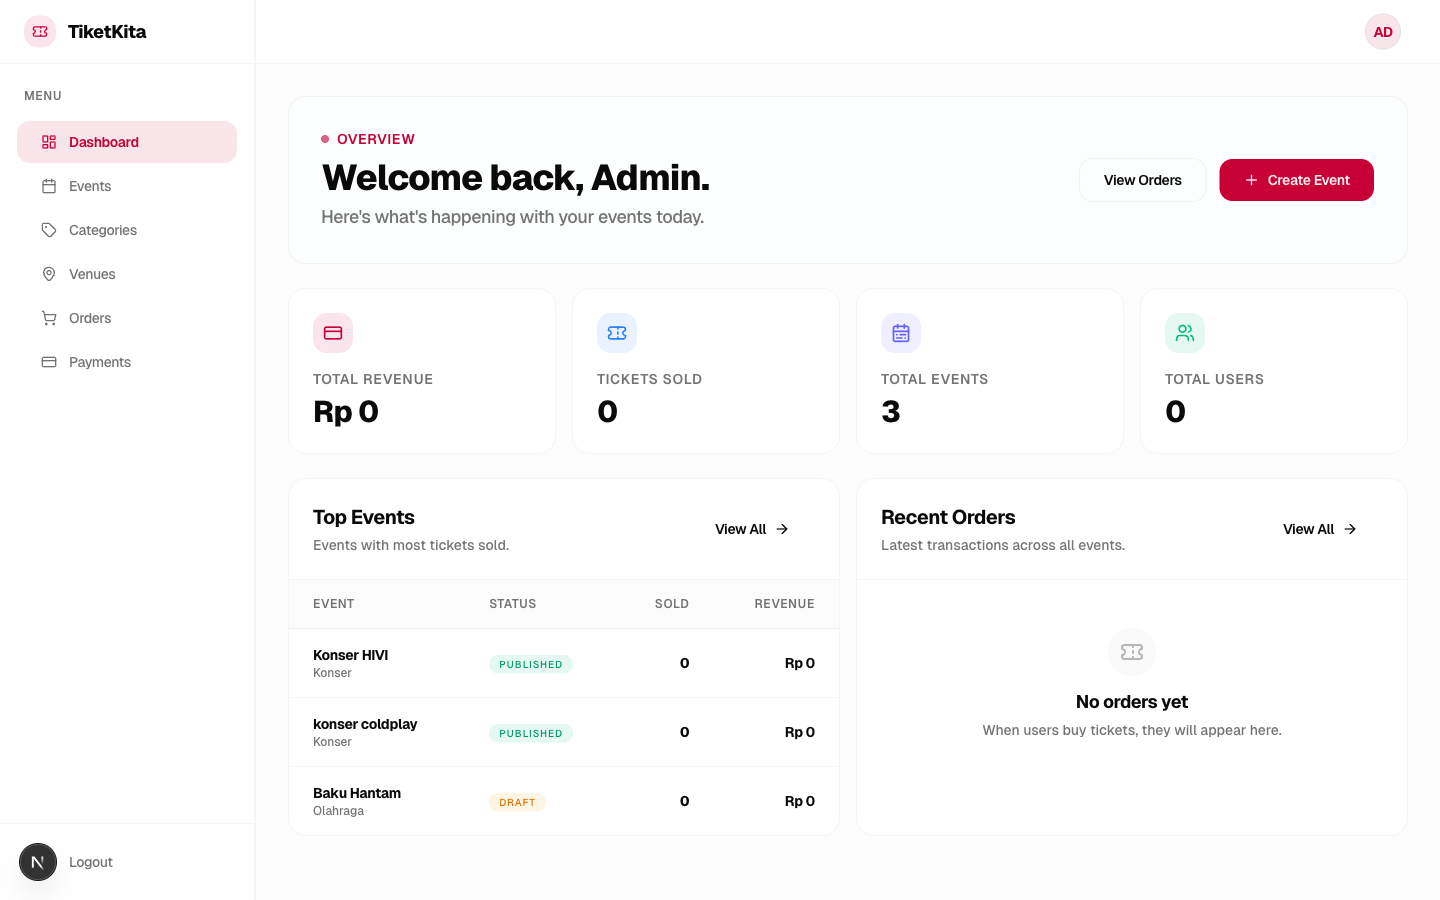
\includegraphics[height=0.4\textheight,keepaspectratio]{screenshots/dashboard.png}
\caption{Tampilan Dashboard Admin}
\label{fig:ss-dashboard}
\end{figure}

\begin{figure}[ht]
\centering
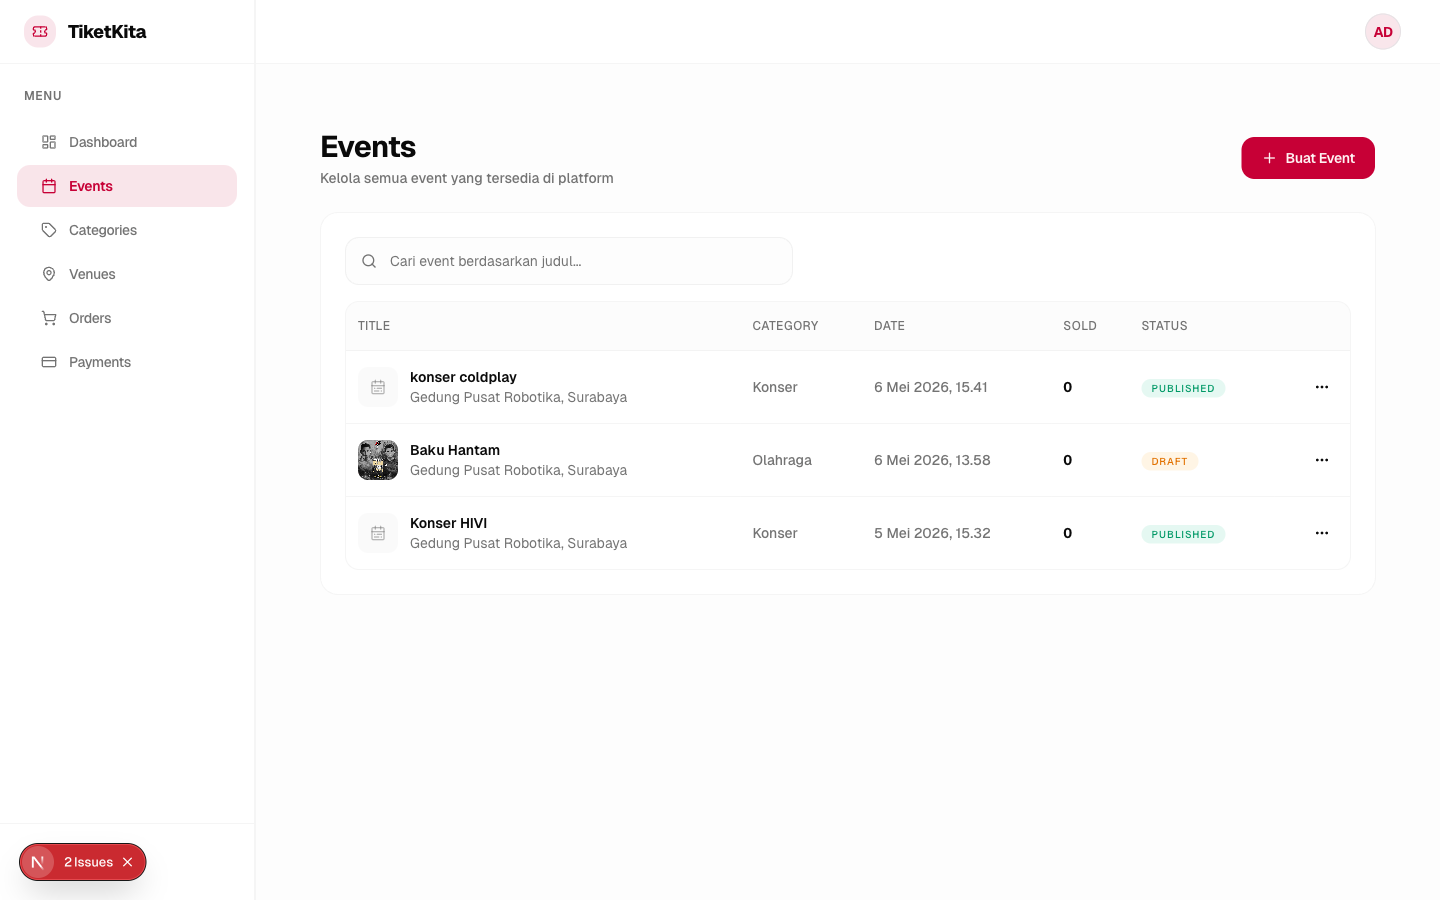
\includegraphics[height=0.4\textheight,keepaspectratio]{screenshots/events-list.png}
\caption{Tampilan Daftar Events}
\label{fig:ss-events-list}
\end{figure}

\begin{figure}[ht]
\centering
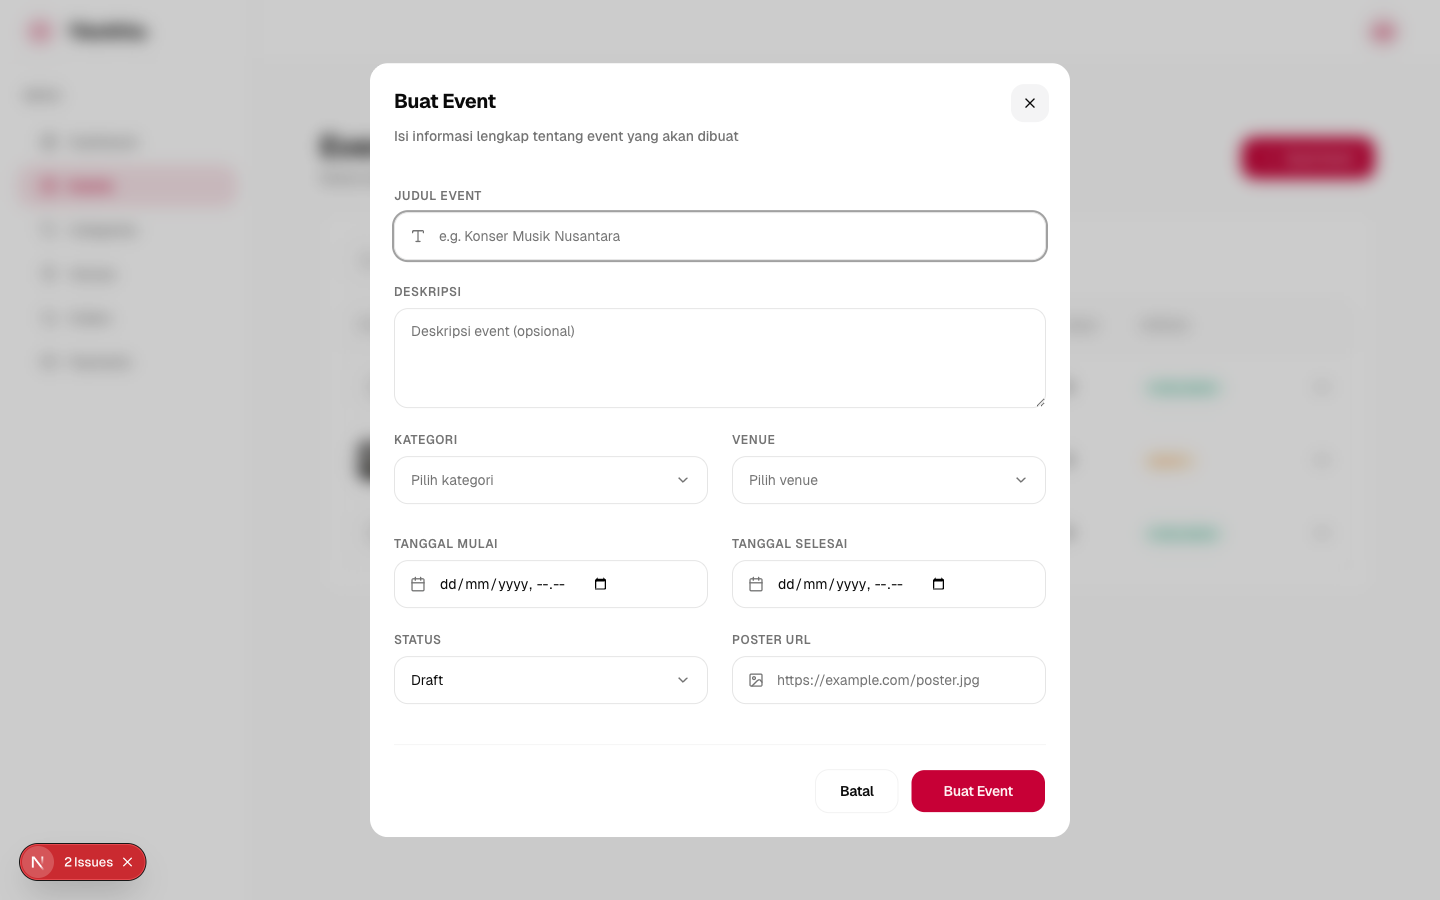
\includegraphics[height=0.4\textheight,keepaspectratio]{screenshots/event-form.png}
\caption{Tampilan Form Create/Edit Event}
\label{fig:ss-event-form}
\end{figure}

\begin{figure}[ht]
\centering
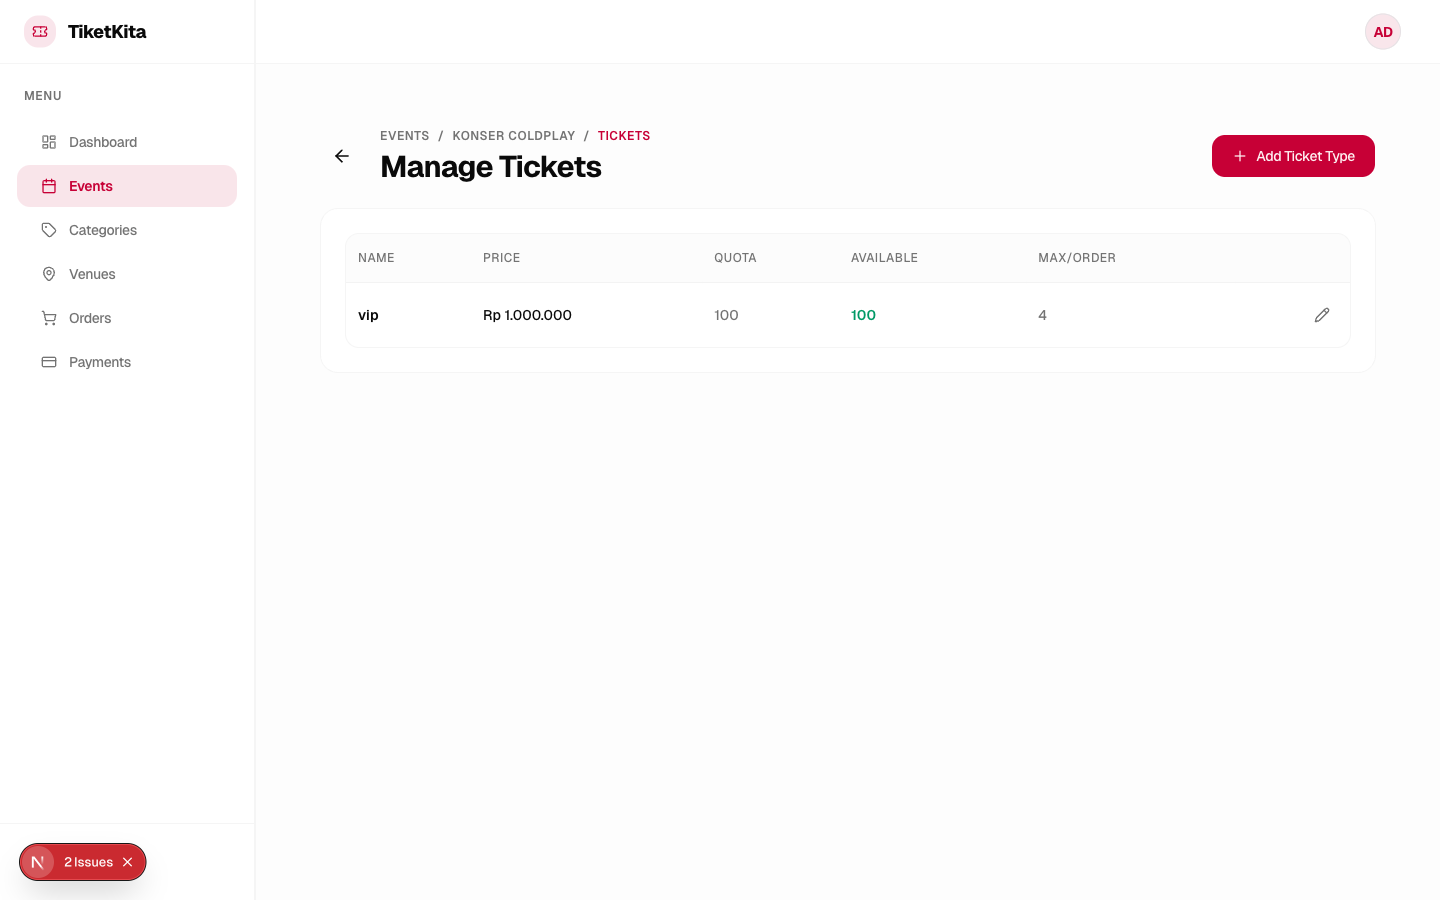
\includegraphics[height=0.4\textheight,keepaspectratio]{screenshots/event-tickets.png}
\caption{Tampilan Manajemen Tipe Tiket per Event}
\label{fig:ss-event-tickets}
\end{figure}

\begin{figure}[ht]
\centering
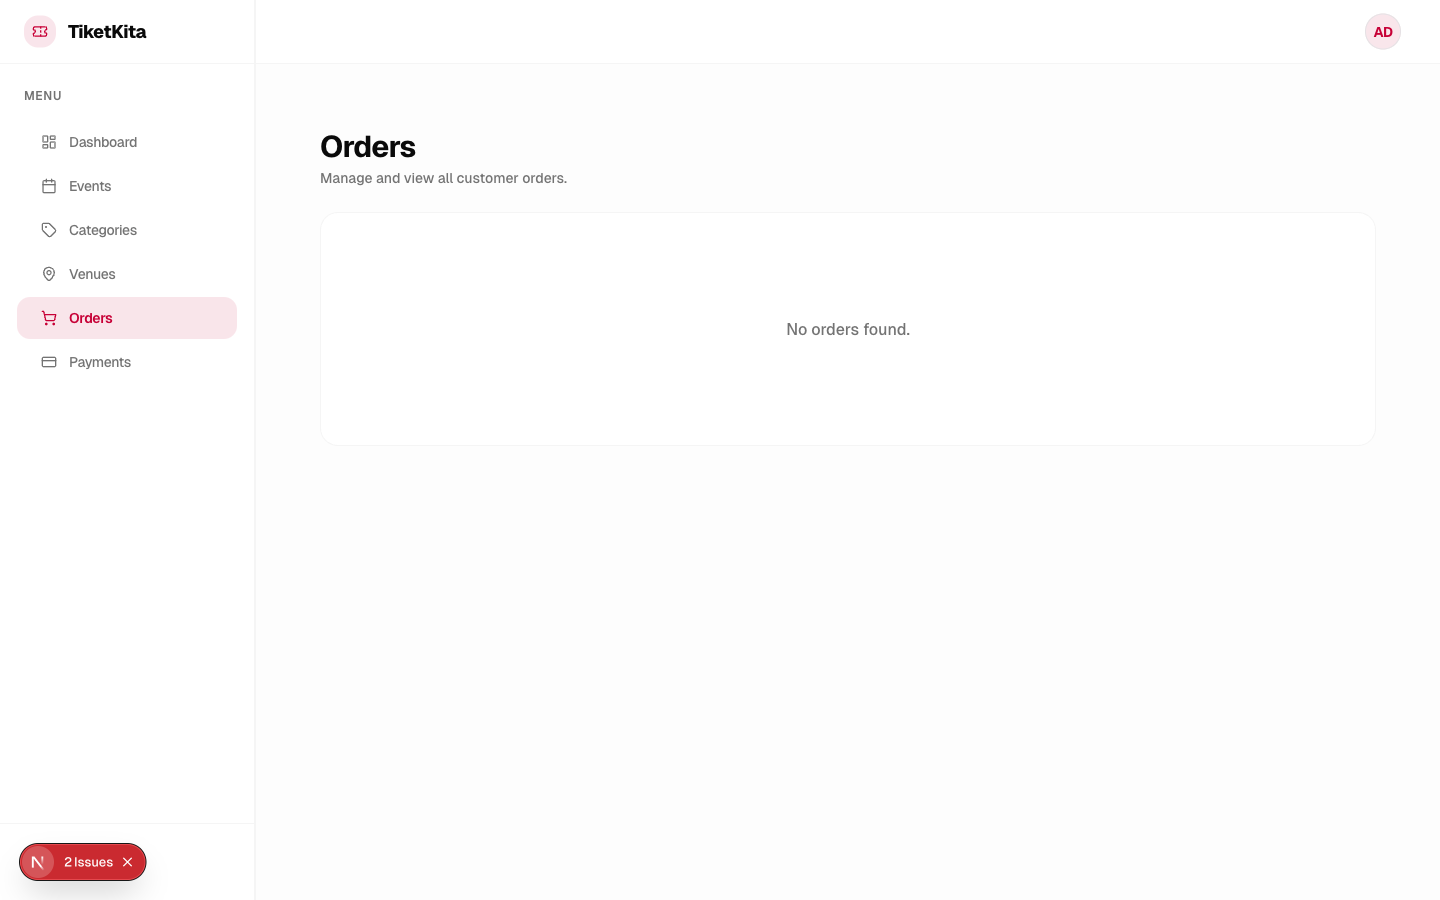
\includegraphics[height=0.4\textheight,keepaspectratio]{screenshots/orders-list.png}
\caption{Tampilan Daftar Order}
\label{fig:ss-orders-list}
\end{figure}

\begin{figure}[ht]
\centering
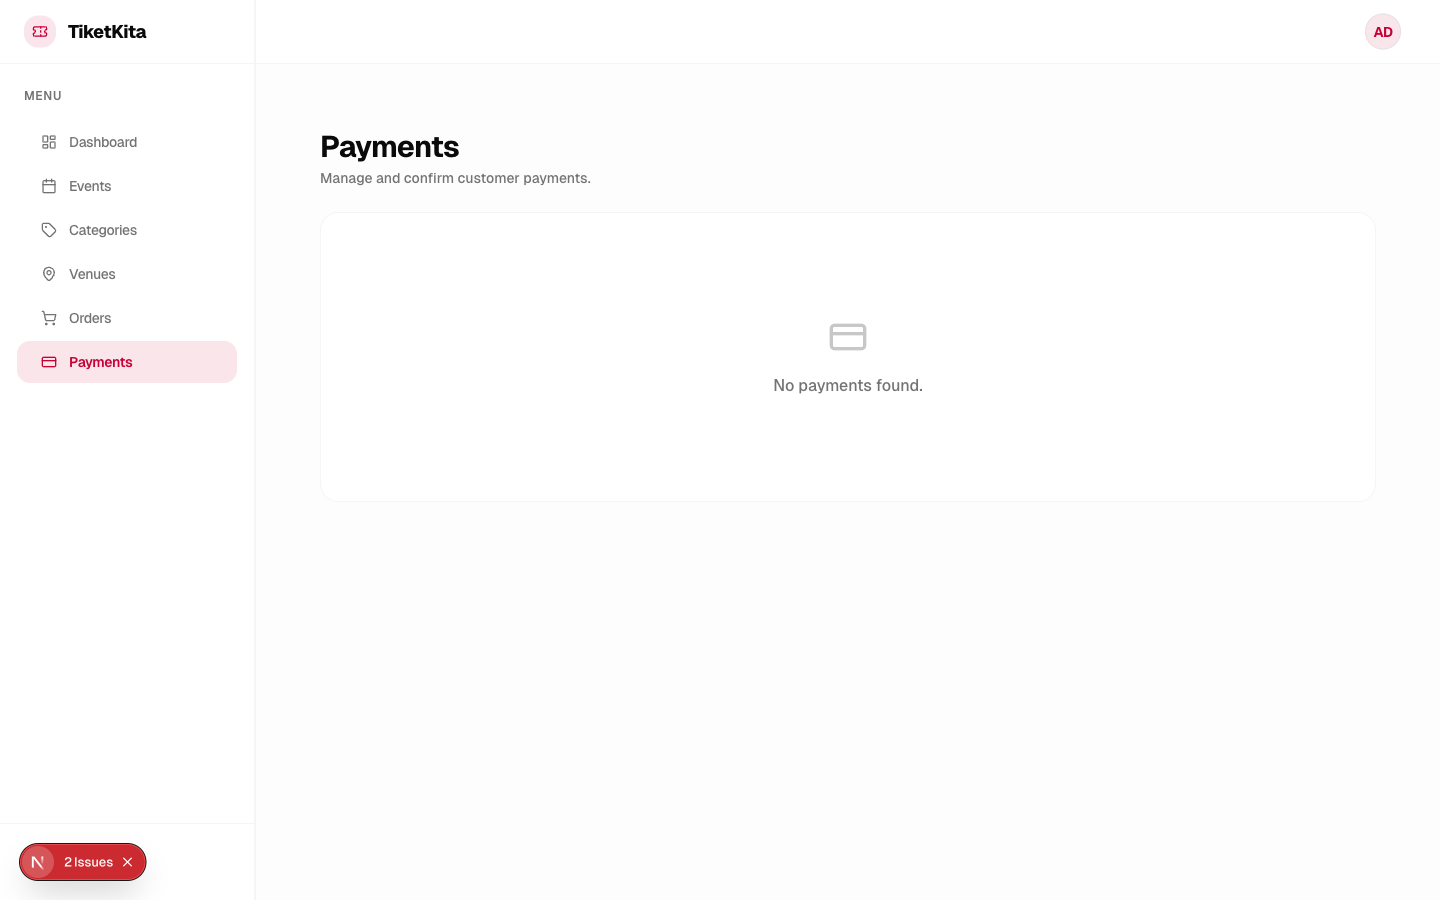
\includegraphics[height=0.4\textheight,keepaspectratio]{screenshots/payments.png}
\caption{Tampilan Konfirmasi Pembayaran}
\label{fig:ss-payments}
\end{figure}

\begin{figure}[ht]
\centering
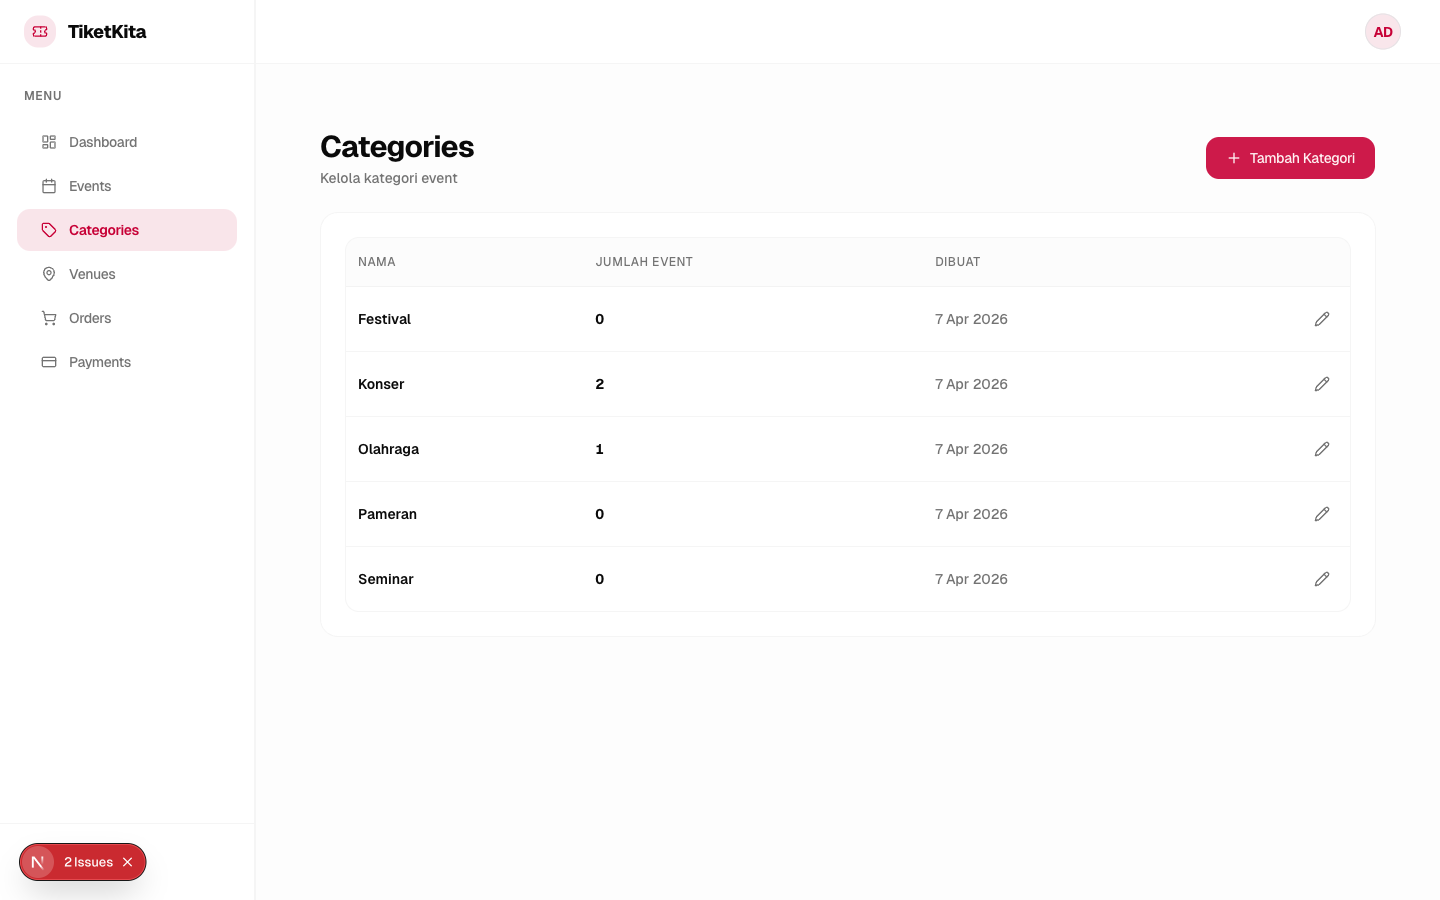
\includegraphics[height=0.4\textheight,keepaspectratio]{screenshots/categories.png}
\caption{Tampilan Manajemen Kategori}
\label{fig:ss-categories}
\end{figure}

\begin{figure}[ht]
\centering
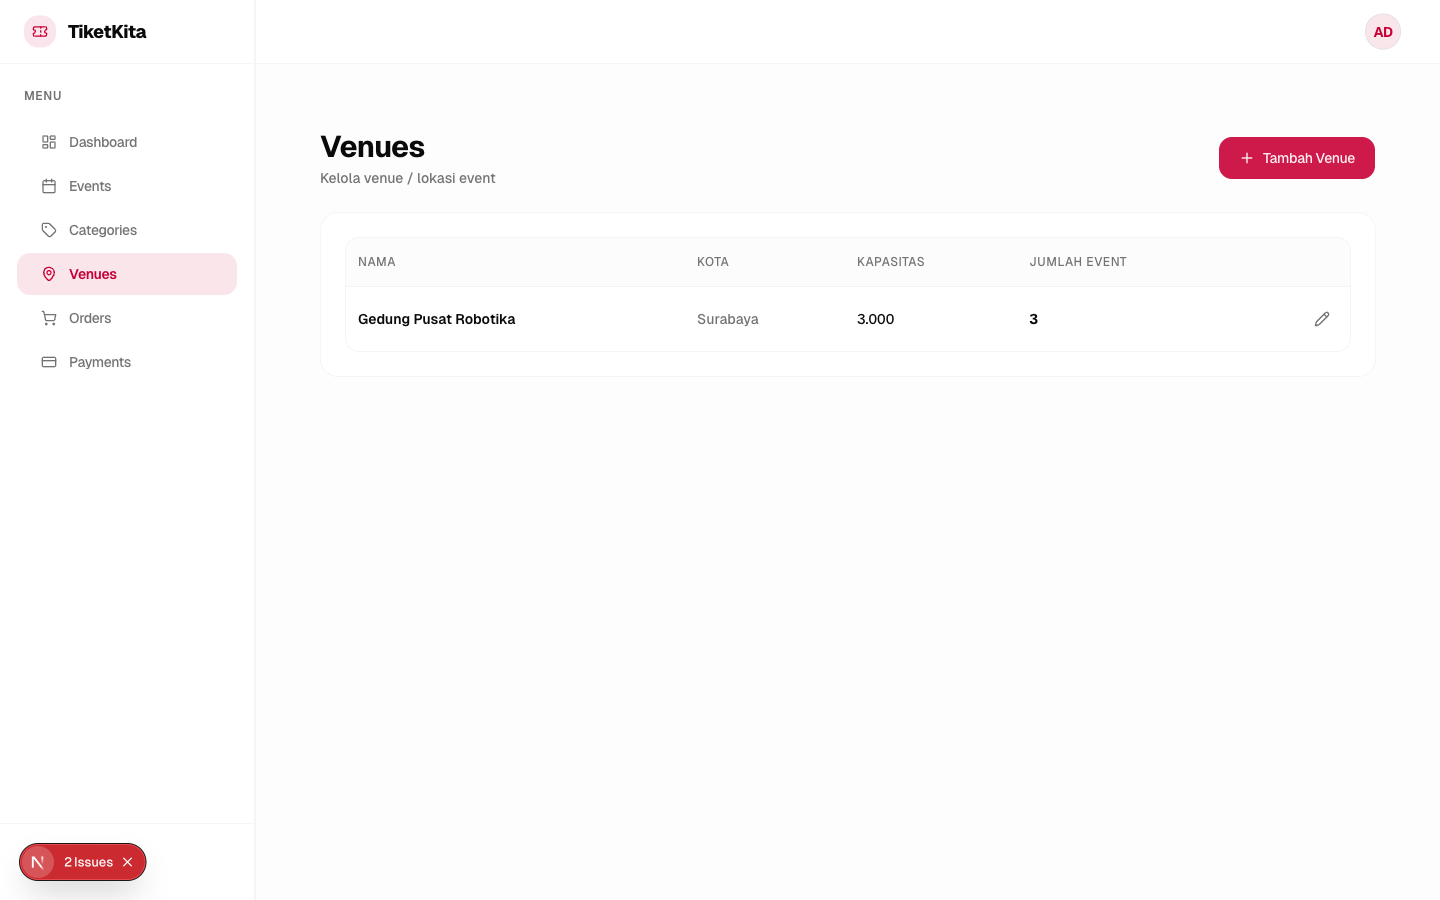
\includegraphics[height=0.4\textheight,keepaspectratio]{screenshots/venues.png}
\caption{Tampilan Manajemen Venue}
\label{fig:ss-venues}
\end{figure}

\begin{figure}[ht]
\centering
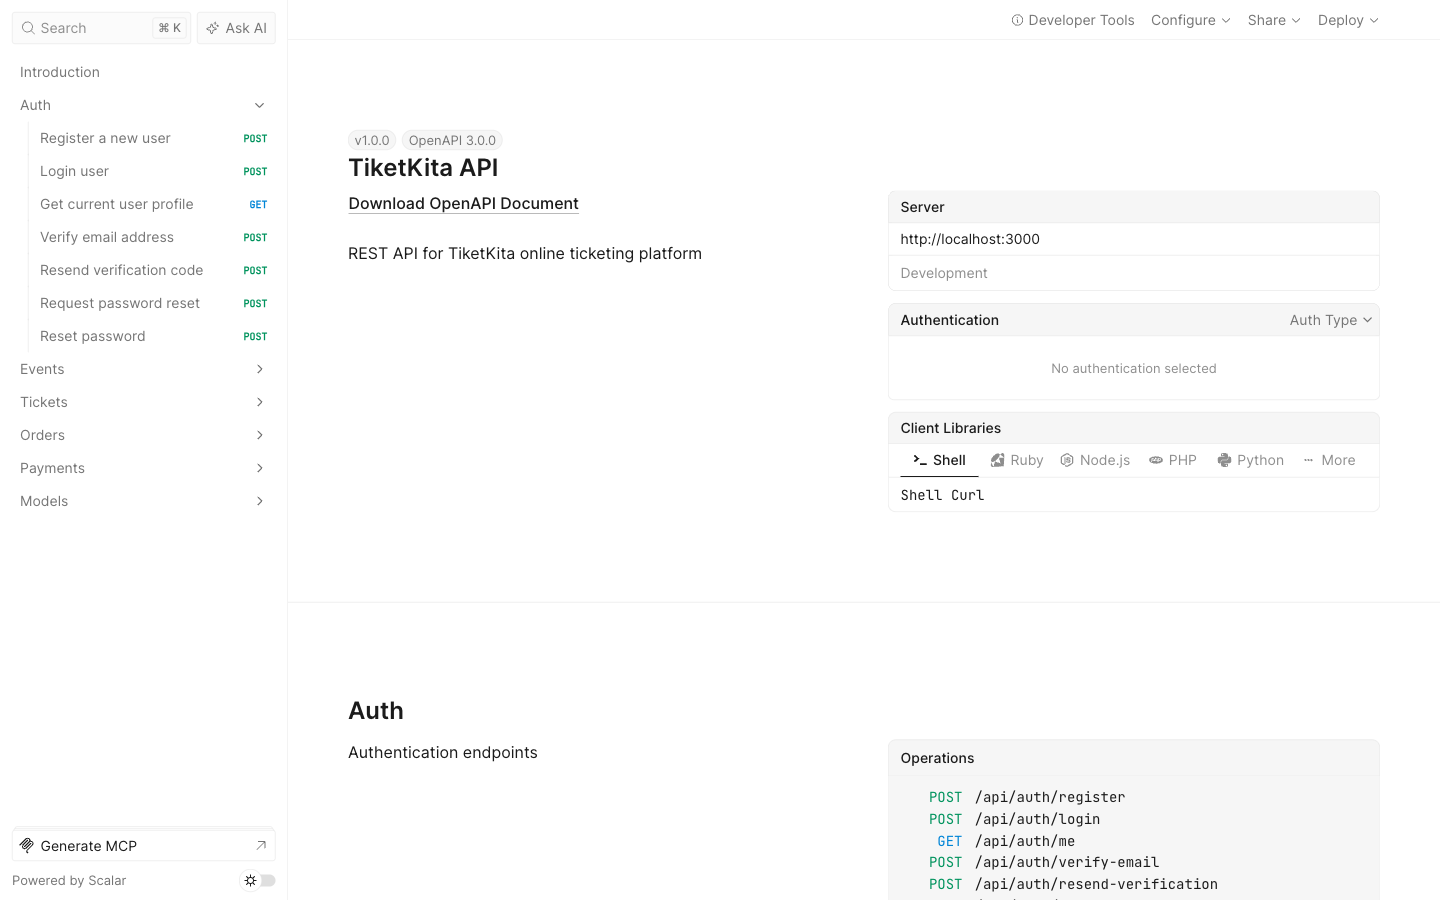
\includegraphics[height=0.4\textheight,keepaspectratio]{screenshots/api-docs.png}
\caption{Dokumentasi API Interaktif via Scalar pada \texttt{/api/docs}}
\label{fig:ss-api-docs}
\end{figure}

\section{Progress Checklist}
Tabel \ref{tab:progress-checklist} merangkum status pengerjaan setiap komponen utama proyek pada tahap progres ini.

\begin{table}[h]
\centering
\caption{Progress Checklist Pengerjaan}
\label{tab:progress-checklist}
\begin{tabular}{lc}
\toprule
\textbf{Komponen} & \textbf{Status} \\
\midrule
Backend REST API (11 modul)        & $\checkmark$ Selesai \\
Migrasi Database (14 file)         & $\checkmark$ Selesai \\
Seed Data                          & $\checkmark$ Selesai \\
Dokumentasi API (Scalar)           & $\checkmark$ Selesai \\
Dashboard Admin (10 halaman)       & $\checkmark$ Selesai \\
CRUD Promo Codes (Admin)           & $\circ$ Dalam Pengerjaan \\
Frontend Publik/Customer           & $\times$ Belum Dimulai \\
Integrasi Payment Gateway          & $\times$ Belum Dimulai \\
Deployment Production              & $\times$ Belum Dimulai \\
\bottomrule
\end{tabular}
\end{table}

%======================================================================
% BAB V PENUTUP
%======================================================================
\chapter{Penutup}

\section{Kesimpulan}
Pada tahap progres ini, tim telah berhasil menyelesaikan komponen inti dari platform TiketKita. Backend REST API dengan sebelas modul fungsional telah berjalan di atas basis data MySQL yang terdiri dari sebelas tabel ternormalisasi, lengkap dengan sistem migrasi dan seed data. Dashboard administrator dengan sepuluh halaman juga telah berfungsi penuh untuk pengelolaan event, tipe tiket, order, pembayaran, kategori, dan venue, sementara dokumentasi API otomatis telah disediakan melalui Scalar pada endpoint \texttt{/api/docs}.

Capaian tersebut telah memenuhi keempat tujuan yang dirumuskan pada BAB I. Skema basis data relasional ternormalisasi telah dirancang dan diimplementasikan, mekanisme transaksi MySQL telah memastikan konsistensi data pada alur pemesanan tiket termasuk pencegahan race condition pada stok, REST API berbasis Node.js dan TypeScript dengan arsitektur Controller-Service-Repository telah berdiri kokoh tanpa ORM, dan dashboard admin berbasis Next.js telah berfungsi sebagai antarmuka pengelolaan data yang informatif. Dengan demikian fondasi sistem sudah cukup matang untuk dilanjutkan pada tahap pengembangan berikutnya.

\section{Rencana Selanjutnya}
\begin{enumerate}
    \item Menyelesaikan fitur CRUD promo codes pada dashboard admin.
    \item Membangun frontend publik/customer-facing untuk alur pemesanan tiket oleh pengguna akhir.
    \item Mengintegrasikan payment gateway nyata (misalnya Midtrans atau Xendit) menggantikan simulasi pembayaran.
    \item Melakukan deployment ke environment production dengan konfigurasi keamanan dan performa yang memadai.
\end{enumerate}

%======================================================================
% DAFTAR PUSTAKA
%======================================================================
\begin{thebibliography}{9}
\bibitem{elmasri2015}
  Elmasri, R. \& Navathe, S.B. (2015).
  \textit{Fundamentals of Database Systems}, 7th ed.
  Pearson Education.

\bibitem{mysql2024}
  Oracle Corporation. (2024).
  \textit{MySQL 8.0 Reference Manual}.
  Tersedia di: \url{https://dev.mysql.com/doc/refman/8.0/en/}

\bibitem{expressjs2024}
  OpenJS Foundation. (2024).
  \textit{Express.js Documentation}.
  Tersedia di: \url{https://expressjs.com/}

\bibitem{nextjs2024}
  Vercel. (2024).
  \textit{Next.js Documentation}.
  Tersedia di: \url{https://nextjs.org/docs}

\bibitem{zod2024}
  Colinhacks. (2024).
  \textit{Zod: TypeScript-first schema validation}.
  Tersedia di: \url{https://zod.dev/}
\end{thebibliography}

\end{document}
